\documentclass[11pt]{amsart}
\usepackage{geometry}                % See geometry.pdf to learn the layout options. There are lots.
\geometry{letterpaper}                   % ... or a4paper or a5paper or ... 
%\geometry{landscape}                % Activate for for rotated page geometry
\usepackage[parfill]{parskip}    % Activate to begin paragraphs with an empty line rather than an indent
\usepackage{graphicx}
\usepackage{amssymb}
\usepackage{epstopdf}
\DeclareGraphicsRule{.tif}{png}{.png}{`convert #1 `dirname #1`/`basename #1 .tif`.png}
\usepackage{amsfonts,amsmath,amsthm,amsbsy,latexsym,amssymb,graphicx,booktabs,multicol,color,fullpage}
\usepackage{mathabx,dashrule}
\usepackage{pgf,tikz}
\usepackage{pgfplots}
\usepackage{graphicx}
\usepackage{wrapfig}
\usepackage{multicol}
\usepackage{arydshln}
\usepackage{verbatim}
\usepackage{xcolor}
\newcommand{\subf}[2]{%
  {\small\begin{tabular}[t]{@{}c@{}}
  #1\\#2
  \end{tabular}}%
}


\title{A Numerically Stable Fourier Continuation Approximation for the Solution of Partial Differential Equations}
\author{Melanie Vining \\ Integrated and Applied Mathematics \\University of New Hampshire}
%\date{}                                           % Activate to display a given date or no date

\begin{document}

\maketitle
\begin{abstract}
Fourier Continuation approximation is a spectral method for function approximation which has proven effective for PDE solution on complex domains. Fourier Continuation solves a least-squares problem to find a periodic extension of the function.  The solution to PDEs on complex domains can be found via Fourier-Continuation combined with an Alternating-Direction approach (FC-AD).  Use of the FC-AD method splits the solution to a PDE into the solutions of a series of one-dimensional Boundary Value Problems (BVPs).  We present a novel approach to find the Fourier Continuation approximations for direct application to the FC-AD method that enforces stability by exploiting the Singular Value Decomposition (SVD) of the Fourier Continuation matrix. Modifying a highly-accurate result for the Fourier Continuation approximation results in stable and still high-order accurate approximations.   
\end{abstract}
\newpage



\section{Introduction} 
\subsection{Motivation} 
The goal is to study a numerically accurate and stable scheme for solving partial differential equations on complex domains.  Several finite difference and finite element methods are available but have low-order accuracy.  We focus on the Fourier-Continuation Alternating-Direction (FC-AD) method described by Bruno and Lyon in \cite{FCAD1},\cite{FCAD2}. This method gives a high-order unconditionally stable solver for partial differential equations on any smooth domain.  One of the interesting details in the FC-AD method is that a certain modification to the solution that yields unconditional stability which is neither inherent to the problem nor an obvious choice and was in fact developed by numerical experiment. The aim is to find an unconditional stability condition that is more natural either to the problem itself and to the mechanics of the implementation.  


\subsubsection{FC-AD}
The Fourier-Continuation Alternating-Direction algorithm is a method that applies the concept of Alternating Direction Implicit (ADI) methods to using a Fourier Continuation (FC) method in the spatial domain.  ADI methods reduce the numerical solution to PDEs into implicit first order boundary value problems in space.  In traditional ADI methods, these  BVPs are solved using finite-difference methods and yield low-accuracy results, particularly on the boundaries.  \\
Given the heat equation in two dimensions:
\begin{eqnarray}
u_t=k(u_{xx}+u_{yy}) + Q(x,y,t), & (x,y,t) \in \Omega \times (0,T], \nonumber \\
u(x,y,t) = G(x,y,t) & (x,y) \in \partial \Omega, t \in (0,T] \\
u(x,y,0)=u_0(x,y), & (x,y) \in \Omega, \nonumber 
\end{eqnarray}
with $k>0$, $\Omega \subset \mathbb{R}^2$ is smoothly bounded, and $Q$, $G$, and $u_0$ are smooth.  Discretizing according to $t^n=n\Delta t$, we then use a central difference scheme for the time derivative and enforce at $t^{n+\frac{1}{2}}=(n+\frac{1}{2})\Delta t$, resulting in
\begin{equation}
\dfrac{u^{n+1}-u^n}{\Delta t} = \dfrac{k}{2}\dfrac{\partial^2}{\partial x^2}(u^{n+1}-u^n) +\dfrac{k}{2}\dfrac{\partial^2}{\partial y^2}(u^{n+1}-u^n) + Q^{n+\frac{1}{2}} + E_1(x,y,\Delta t)
\end{equation}.
Here, $Q^{n+\frac{1}{2}}= Q(x,y,(n+\frac{1}{2})\Delta t)$ and $E_1(x,y,\Delta t)$ is the error term resulting from the central difference differentiation.  
Rearranging this equation yields
\begin{equation}
\left(1-\dfrac{k\Delta t}{2}\dfrac{\partial ^2 }{\partial x ^2 } - \dfrac{k\Delta t}{2}\dfrac{\partial ^2 }{\partial y ^2 }\right)u^{n+1}= \left(1+\dfrac{k\Delta t}{2}\dfrac{\partial ^2 }{\partial x ^2 } + \dfrac{k\Delta t}{2}\dfrac{\partial ^2 }{\partial y ^2 }\right)u^n + Q^{n+\frac{1}{2}}+E_1(x,y,\Delta t)
\end{equation}
and then factoring the left hand side and moving extra terms over gives 

\begin{equation}
\begin{aligned}
\left(1-\dfrac{k\Delta t}{2}\dfrac{\partial ^2}{\partial x^2} \right) \left(1-\dfrac{k\Delta t}{2}\dfrac{\partial ^2}{\partial y^2} \right)u^{n+1}& =  
\left(1+\dfrac{k\Delta t}{2}\dfrac{\partial ^2}{\partial x^2} \right) \left(1+\dfrac{k\Delta t}{2}\dfrac{\partial ^2}{\partial y^2} \right)u^n\\ &+ \dfrac{k^2 \Delta t^2}{4}\dfrac{\partial ^ 2}{\partial x^2}\dfrac{\partial ^2}{\partial y ^ 2} (u^{n+1}-u^n) + \Delta t Q^{n + \frac{1}{2}} + \Delta t E_1(x,y,\Delta t)
\end{aligned}
\end{equation}.

To solve for $u^{n+1}$, the operators on the left side must be inverted, which results in equations of the form 
\begin{eqnarray}
u-\alpha u'' = f, & u(x_{\ell})=B_{\ell}, & u(x_r)=B_r 
\end{eqnarray}
where $\alpha=\dfrac{k\Delta t}{2}$ \cite{FCAD1}.  This turns a 2-D Partial Differential Equation into a sequence of 1-D Boundary Value Problems, which we can solve via whichever method is chosen.  For the FC-AD method, a Fourier Continuation approximation is used to solve the differential equation numerically.  

\subsubsection{Fourier Continuation}
Fourier Series methods for approximating functions are well-known to be accurate on functions that are periodic on a specified interval.  However, in the attempt to approximate non-periodic functions on the same interval using Fourier Series, we see the Gibbs phenomenon and as a result the accuracy that we could have expected in the periodic case is no longer valid.  

The goal of Fourier Continuation approximations is to see the high rate of convergence of Fourier Series in approximating periodic functions and find some way to get the same, or similar rate of convergence for non-periodic functions.  

Given a smooth function $y=f(x)$ on the interval $[0,1]$ (this is arbitrarily chosen for simplicity), with $f\in C^k[0,1]$, where $k \in \mathbb{Z}^{+}$ or $k=\infty$, let $x_j$, $j=1 \ldots N$ be the discretization of the interval $[0,1]$ onto $N$ points and let $y_j  = f(x_j)$.  
The goal is to interpolate the points $(x_j,y_j)$ in terms of trigonometric polynomials with period $b>1$ with $M$ Fourier Modes, $M<N$.  
In essence, the resulting overdetermined system needs to be solved:
\begin{eqnarray}
y_j=\sum_{k\in t(M)} a_k e^{\dfrac{2\pi i}{b}kx_j}, &j=1\ldots N
\end{eqnarray}
where $t(M)=\{j\in \mathbb{N}: -(M-1)/2 \leq j \leq (M-1)/2\}$ if $M$ is odd and $t(M)=\{j\in \mathbb{N}: -M/2\leq j \leq M/2-1\}$ if $M$ is even. 
Traditionally, this system is split into sines and cosines and solved via least-squares methods\cite{FC1}.  




\subsubsection{FC Gram}
The FC Gram method matches points on a grid and applies a precomputed extension that results in a periodic function.  This resulting function can then be transformed via Fast Fourier Transform (FFT) in order to take derivatives. 

To begin, start with a basis of functions, $f_0,f_1,\ldots,f_{n-1}$.  These functions can be any functions, but having an orthogonal basis or an orthonormal basis makes future computations  and theoretical considerations much simpler.  Using the Gram Polynomials is a natural option for this particular application of FC-Gram due to the equispaced points prescribed by the FC-AD Method.   These can be computed as point values using the desired grid via a QR factorization on a Vandermonde matrix.  
 
Then approximations with periodic extensions are then calculated for each function for a predetermined number of points $n$, giving us $f_{0_c},f_{1_c},\ldots f_{n-1_c}$.  Specifically, it makes sense to use the periodic extensions found when using the Fourier Continuation approximation method, hence the ``FC" in FC-Gram.  These approximations are stored as a basis.  

Next, the approximations need to be matched to the function.  Given a function $f$ defined on $m \geq n$ points, we consider the first $n$ points and the last $n$ points of the function (noting that if $m=n$, these will be the same points and overlap is permitted). We then fit the first $n$ points to the basis and the last $n$ points to the basis separately, giving us $a_1$ and $a_2$.  Then an appropriate combination of $a_1$ and $a_2$ is taken to get a smooth, periodic extension of $f$.  This periodic extension has a rapidly convergent Fourier Series and can be used in applications going forward, while preserving the original data.   

\section{Current Work}
As a result of the FC-AD method, we study the Boundary Value Problem (BVP) $-\alpha u'' + u=f$ with boundary values $u(a)=u_a$ and $u(b)=u_b$.  The goal is to find the ``best" Fourier Continuation approximation that can be used to approximate $f$ such that when the operator is inverted to solve for $\tilde{u}$ (numerically), the result is stable, i.e. $\frac{\|\tilde{u}\|_{\ell^2}}{\|\tilde{f}\|_{\ell^2}} \leq 1$.  \\
The trouble that follows (or the problem that is considered below) is that the Fourier Continuation approximation can take any form in the continuation domain, as long as the result has the desired accuracy (see Figure \ref{fig:Fig1}). \\
\begin{figure}[h!]
\begin{center}
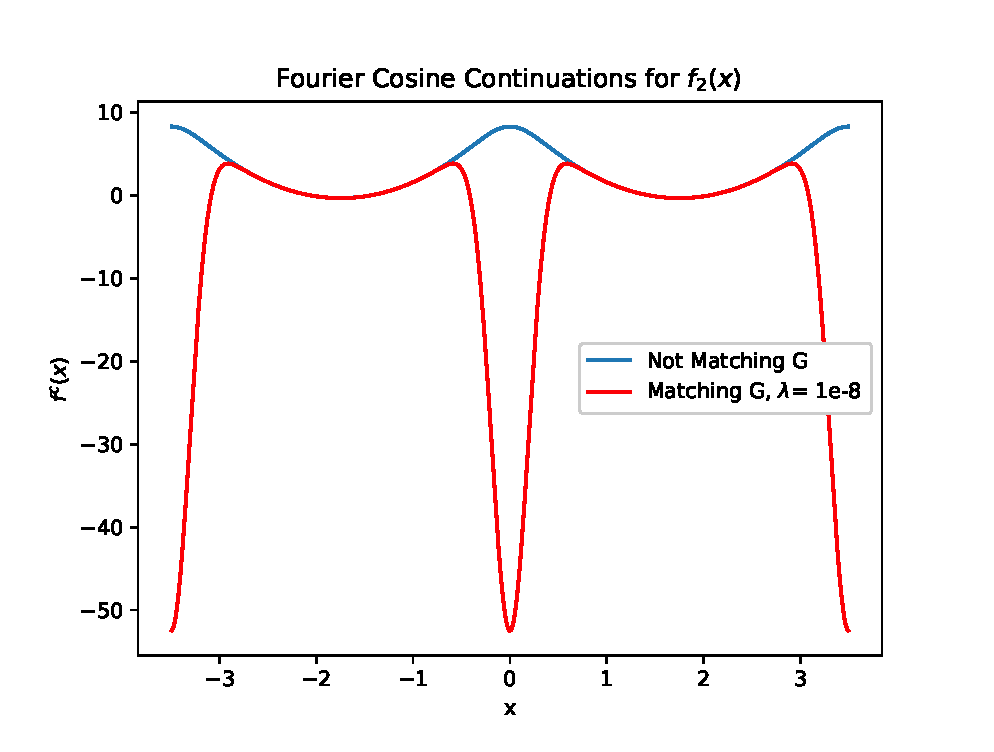
\includegraphics[scale = .7]{f_2ForComparison.eps}
\caption{Two different Fourier Continuations for a degree 2 polynomial. Both give approximately 17 digits of accuracy.}
\label{fig:Fig1}
\end{center}
\end{figure}
This means that it is possible for a procedure to ``choose" a Fourier Continuation approximation for which energy builds in the continuation region, and then will spread back into the original domain under the inverted operator.  In practice, this gives an unstable result.  In Figure \ref{fig:Fig1} we see that for no trade in accuracy, the blue line gives us an unstable result, while the red line gives a stable result. \\

\subsection{What We've Done} 
The Singular Value Decomposition (SVD) of the system was explorted in order to try to exploit the zero singular values, but that proved to be ineffective in changing the shape of the continuation due to horrible conditioning of the system($\texttt{cond(A)}=\mathcal{O}(10^{17})$)  and the inherent constraints that we were forced to impose upon it. 

It was determined that by adding extra constraints to the system being solved, there would be more control over the system in question. Some fruitful results have come from focusing on a known solution to the BVP: The Green's Function. For simplicity, assume that $a=-1$ and $b=b$ and that there are zero Boundary Conditions (BCs). 
\begin{comment}
 \subsubsection{Green's Functions}
The Green's Function solution was then calculated via the methods described in Bender and Orszag: Let 
\begin{equation}
G(x,a)=\begin{cases}
A_1(a)h_1(x)+B_1(a)h_2(x) & x<a \\
A_2(a)h_1(x)+B_2(a)h_2(x) & x \geq a
\end{cases}
\end{equation}
where $h_1(x)$ and $h_2(x)$ are the homogeneous solutions to  $(I-\alpha \frac{\partial^2}{\partial x^2})u=f$:

\begin{eqnarray}
h_1(x) &=& e^{\frac{(x-b)}{\sqrt{\alpha}}} \\
h_2(x) &=& e^{\frac{(-x-1)}{\sqrt{\alpha}}},
\end{eqnarray}

where $h_1$ and $h_2$ have been normalized to $1$ on the boundary.  $A_1$,$A_2$,$B_1$, and $B_2$ are computed to enforce continuity of the Green's Function, at most a small jump discontinuity of the Green's Function, and zero boundary conditions \cite{BO}.  The Green's Function for our BVP ends up being

\begin{equation}
G(x,a)=\begin{cases} 
-\dfrac{1}{2} \dfrac{\sqrt{\alpha}\left(-e^{\frac{-1-2b+a}{\sqrt{\alpha}}}+e^{-\frac{a+1}{\sqrt{\alpha}}}\right)\left(-e^{\frac{2(2+b+x)}{\sqrt{\alpha}}}+e^{\frac{2(x+1)}{\sqrt{\alpha}}}+e^{\frac{2(1+b)}{\sqrt{\alpha}}}-1\right)e^{\frac{-x+1+2b}{\sqrt{\alpha}}}}{\left(e^{\frac{2(1+b)}{\sqrt{\alpha}}}-1\right)^2} & x<a \\
\dfrac{1}{2} \dfrac{\sqrt{\alpha} \left(e^{\frac{2+b+a}{\sqrt{\alpha}}} -e^{\frac{a-b}{\sqrt{\alpha}}}\right)\left(e^{\frac{2(-x+b)}{\sqrt{\alpha}}}+e^{\frac{2(1+b)}{\sqrt{\alpha}}}-e^{\frac{2+4b-2x}{\sqrt{\alpha}}}-1\right)e^{\frac{2+b+x}{\sqrt{\alpha}}}}{\left(e^{\frac{2(1+p)}{\sqrt{\alpha}}}-1\right)^2} & x \geq a

\end{cases}
\end{equation}

The final calculation of the Green's Function solution to the BVP comes from the convolution integral
\begin{equation}
u_G=\int_{-1}^b G(x,a)f(a)da.
\end{equation}
where $u_G(x)$ is the Green's Function solution for given $f(x)$.
\end{comment}


\subsubsection{System of Equations}

Starting with $n$ points, the number of points desired on the coarse grid, and the minimal number of points needed to perform the FC-Gram computations, consider $x \in [-1, 1-\dfrac{2}{n}]$.  Splitting this interval into $n$ equispaced points gives us $\{x_j\}_{j=0}^9$.  We then compute the coefficients for the Gram Polynomials $f_0,f_1,\ldots f_9$(and their point values on the grid) by computing the QR factorization of the Vandermonde matrix of $\{x_j\}$.  While having the point values is enough if we were using a coarse grid, we need the coefficients of the polynomials both to compute the point values on a fine grid and also to compute the Green's Function solution.  


A finer grid is also constructed, $\tilde{x}$.  We choose the fine grid to be $F$ times more refined than the coarse grid, giving $h_f=\dfrac{h}{F}$.  Using the coefficients, the Gram Polynomials were calculated first as symbolic expressions, and then evaluated on the fine grid, giving  $\tilde{f}_0,\tilde{f}_1,\ldots \tilde{f}_9 $.  also construct the homogeneous solutions, $h_1(x)$ and $h_2(x)$, and evaluate them on the fine grid, giving us $\tilde{h}_1$ and $\tilde{h}_2$.  

Next, the Green's Function solution is computed for the given Gram Polynomial and the solution is evaluated on the fine grid. The Green's Function solutions for the monomials were computed symbolically using Maple and the expressions for these solutions were stored.  Using the linearity of integration, the Green's Function solutions were multiplied by the coefficients of the Gram Polynomials and added together,  then  the expressions were evaluated on $\tilde{x}$.  The evaluated Green's Function solutions are labelled  $\tilde{G}_0,\tilde{G}_1,\ldots,\tilde{G}_9$.  Here, $\tilde{G}_j$ depends both on the degree of the polynomial used and on $\alpha$. 

Next we compute the Fourier Continuation matrix.  In our first attempt we used complex exponentials (i.e. we constructed an $n \times n$ Discrete Fourier Transform matrix from $0$ to $2\pi$), however, because of the ill-conditioning of the system, error propagation ruined the preservation of even and odd modes depending on our desire for an even or odd continuation.  

To compute our Continuation Matrix, we start with our desire to have period $B$ (i.e. a period of $B$ times the original length). For our coarse grid, we use $n$ points on an interval of length 1, giving us step size $h_c=\dfrac{1}{n-1}$.  To continue this,  there will be  
\begin{equation}
L_d=(n-1)\times B \times 2
\end{equation}
 points for a double period continuation - one of the boundary points will not be included as it will be repeated.  The stability for the result is calculated on the coarse grid, so the number of points on the coarse grid gives a constraint for the number of modes we are able to use.  We choose to use 
 \begin{equation}
 M=\begin{cases}
 \texttt{floor}(\frac{L_d}{2}-1), & \text{Cosine} \\
 \texttt{floor}(\frac{L_d}{2}-2), & \text{Sine}
 \end{cases}
 \end{equation}
 modes for our expansions, noting that the cosine expansion includes the 0 mode, which is a little less than half the total number of coarse grid points used. 

We construct a fine grid of step size $h_f=\dfrac{h_c}{F}$ ($F$ times more refined than the original coarse grid) and get 
\begin{equation}
F_u=(n-1)\times F + 1
\end{equation} points on the unit length interval and 
\begin{equation}
F_e=(n-1)\times F \times B \times 2
\end{equation} points on our full double period interval (again, we don't include the very last point on the interval as it will get repeated). 

A discrete cosine transform (DCT) matrix is constructed on the fine grid over both the unit interval and on the extended interval, called $C_u$ and $C_e$ respectively.  $C_u$ should have $F_u$ rows and $M$ columns and $C_e$ should have $F_e$ rows and $M$ columns.  Similarly, we construct a discrete sine transform (DST) matrix on both the unite and extended fine grids, and call them $S_u$ and $S_e$ respectively, whose dimensions will be $F_u \times M$ and $F_e \times M$ for the appropriate $M$-value for sine.  It should be noted that both matrices operate from the space of modes and transform into point values.   

We now have a matrix  which we can use to express any function on the correct interval in terms of either a sine or cosine series with period $B$ over $M$ modes.  

Trying to create the cosine continuation for $f$ is the equivalent of solving
\begin{equation}
\min ||C_u f^c - \tilde{f} ||^2 .
\end{equation}
This would yield the coefficients $f^c$ for the Fourier Continuation approximation for $\tilde{f}$.  However, due to the unreliability of the system in terms of stability, additional constraints must be applied.  

This is where we diverge from previous literature.  Instead of experimenting numerically or pre-conditioning our data, instead the Green's function solution is used to hopefully constrain the system in order get a continuation that is stable under the given operator.  

From the differential operator of the BVP, a numerical differential operator can be constructed to represent $I-\alpha \dfrac{\partial ^2 }{\partial x^2}$ for both the sine and cosine transforms, noting that two different differential operators are used due to the difference in number of modes used for sine and cosine, $D_c$ and $D_s$. Then the inverted differential operator is applied to the Fourier Continuation coefficients, and then evaluated on point values using the continuation matrices. This is forced to match the point values of the Green's Function solution.

This adds a new constraint to our problem: 
\begin{equation}
\min ||C_u f^c - \tilde{f}|| ^2 + ||C_u D_c^{\dagger} f^c - \tilde{G}||^2
\end{equation} 

In this computation, it was discovered that the homogeneous solutions are not well-represented in terms of the cosine or sine basis, so the pieces of the homogeneous solutions that contribute to the Green's function solution will not be reached in solving this system, giving rise to high inaccuracy and also pulling away from the desired stability. To remedy this, the inverted differential operator is allowed to be modified by some linear combination of the homogeneous solutions.  This gives additional degrees of freedom to the system and also attempts to remove the dependence of the Green's function on functions that can't be represented in the Fourier bases.  

The system then becomes
\begin{equation}
\min ||C_u f^c - \tilde{f}|| ^2 + ||C_u D_c^{\dagger} f^c +c_1 \tilde{h_1} + c_2 \tilde{h_2} - \tilde{G}||^2
\end{equation}
where the constants $c_1$, $c_2$ are freely chosen by whichever algorithm is used to solve the system.  We use the SVD, which will minimize all of the coefficients it solves for, so we expect $c_1$ and $c_2$ to be (relatively) small.  


Adding this gives rise to great accuracy for both $f^c$ and the solution $u^c$ and almost-stability.  Two more constraints were added to the system in order to achieve stability: first, a parameter $\lambda$ which helps the algorithm to choose smaller values for $c_1$ and $c_2$,  which in turn allows our system to minimize the coefficients $f^c$. To implement this, we let $\lambda c_1 \tilde{h_1} + \lambda c_2 \tilde{h_2} = \bar{0}$, or in our system:
\begin{equation}
\min ||C_u f^c - \tilde{f}|| ^2 + ||C_u D_c^{\dagger} f^c +c_1\tilde{h_1}+c_2\tilde{h_2}- \tilde{G}||^2 + \lambda^2|| c_1 \tilde{h_1} + c_2 \tilde{h_2} ||^2.
\end{equation}

Using $\lambda$ affects the accuracy slightly but gives stability for every polynomial, for any value of $\alpha$.  

Stability can also be enforced by means of another parameter $\mu$ which is applied strictly to the inverted differential operator, but only on points that match with the coarse grid (since stability is computed only on the coarse grid), and the final system to solve becomes
\begin{equation}
\min ||C_u f^c - \tilde{f}|| ^2 + ||C_u D_c^{\dagger} f^c +c_1\tilde{h_1}+c_2\tilde{h_2}- \tilde{G}||^2 + \lambda^2|| c_1 \tilde{h_1} + c_2 \tilde{h_2} ||^2 + \mu^2||C_u D_c^{\dagger}|{\text{\tiny{coarse}}}  ||^2
\end{equation}


\subsection{Implementation}
We chose to implement the solver in the Julia computing language.  This choice was made because Julia has a storage type \texttt{BigFloat} which allows for arbitrary precision as opposed to the double-precision (64-bit).  Setting the precision in Julia to 200 bits allows calculations to be performed with an accuracy of approximately $\mathcal{O}(10^{-77})$, so even losing digits due to round-off error in solving the system, still yields a very high-accuracy result.  Using Julia packages \texttt{LinearAlgebra}, \texttt{SymPy}, \texttt{GenericSVD} and several proprietary functions,  the system above was created and solved using a singular value decomposition and pseudoinverses with a tolerance of $10^{-40}$.  

The matrix used to solve the minimization problem is:
\begin{equation}
\begin{bmatrix}
C_u & \mathbf{0} & \mathbf{0}\\
C_u D_c^{\dagger} & \tilde{h_1} & \tilde{h_2} \\
\mathbf{0} & \lambda \tilde{h_1} & \lambda \tilde{h_2} \\
\mu C_u D_c^{\dagger}|_{\text{\tiny{coarse}}} & \mathbf{0} & \mathbf{0}
\end{bmatrix}
\begin{bmatrix}
f^c \\
c_1\\
c_2
\end{bmatrix}
= 
\begin{bmatrix}
\tilde{f} \\
\tilde{G}\\
\mathbf{0}\\
\mathbf{0}
\end{bmatrix}
\end{equation}.  

Using the psuedoinverse of this matrix with a tolerance of $1e-40$ gives enough accuracy despite having condition numbers $\mathcal{O}(10^{17})$.  

For the computations made, we chose $n=10$ and $B=3.5$, and tested values of $\alpha$ ranging from $0.001$ to $1$.  

\subsection{Error Estimation}
When approximating a function $f$ using an orthogonal set of $n$ polynomials $\Phi_0$, $\Phi_1$, $\ldots$, $\Phi_{n-1}$ , we expect the error between the function $f$ and its approximation $\hat{f}$ to behave like
\begin{equation}
||f-\hat{f}|| = h^0 E_0 + h^1 E_1 + \ldots + h^{n-1} E_{n-1},
\end{equation} 
where $E_0$-$E_{n-1}$ are defined as $||\Phi_i-\hat{\Phi}_i||$ and are known, and the value of $h$ is determined by the accuracy desired. 
Assuming the highest degree polynomial will have the largest error, $h^{n-1}E_{n-1}$ can be used to find the value of $h$. 
(For example, if using a set of $n=10$ orthogonal polynomials, with an error $E_9=1e-2$, if 16 digits of accuracy are desired for the approximation of $f$, $h^9 E_9  = 1e-16$, giving us $h^9=1e-14$ or $h\approx 3e-2$.  Using this, in order to maintain an accuracy of 1e-16, for the 4th degree polynomial the term $h^4E_4$ must also equal $1e-16$, so $E_4$ must be approximately $1e-10$).  \\Operating within these bounds, it can be seen that high accuracy is needed in the lower degree polynomials, but that higher accuracy in the higher degree polynomials will not affect the overall accuracy of the approximation.  \\
Thus, instead of enforcing a strict machine-precision tolerance to approximate each polynomial, the tolerance is relaxed.  This appears in the SVD solve of the system of equations.  By relaxing the tolerance, some of the high-frequency modes which would cause the continuations to grow larger over a shorter interval are taken out of the system.  This controls the size of the continuations and allows for the transition from high precision to double precision without loss of accuracy.  

\subsection{Results} 
Fourier Continuations for all of the polynomials from degree 0 to degree 9 (maximal on 10 points) were calculated.  First, continuations were considered with $\mu=0$, using $\lambda$ to control stability. Stability was observed as a function of $\lambda$, subject to changes in accuracy.   For lower degree polynomials, where accuracy is very high, the use of $\lambda$ is imperative and the use of $\mu$ is seemingly unnecessary.  However, for higher degree polynomials, the accuracy of the continuation is very sensitive to changes in $\lambda$ and sometimes using $\mu$ is more efficient for controlling stability.  

To begin, a simple bisection method was used to compute an optimal value of $\lambda$ which would give rise to the most accuracy while enforcing a stability that was at least $1-\alpha^4$.  

Here are the Cosine continuations for all 10 polynomials with constraint on $\lambda$, for $\alpha =0.001$:  
\begin{figure}[h!]
\centering
\begin{tabular}{|c|c|}
\hline
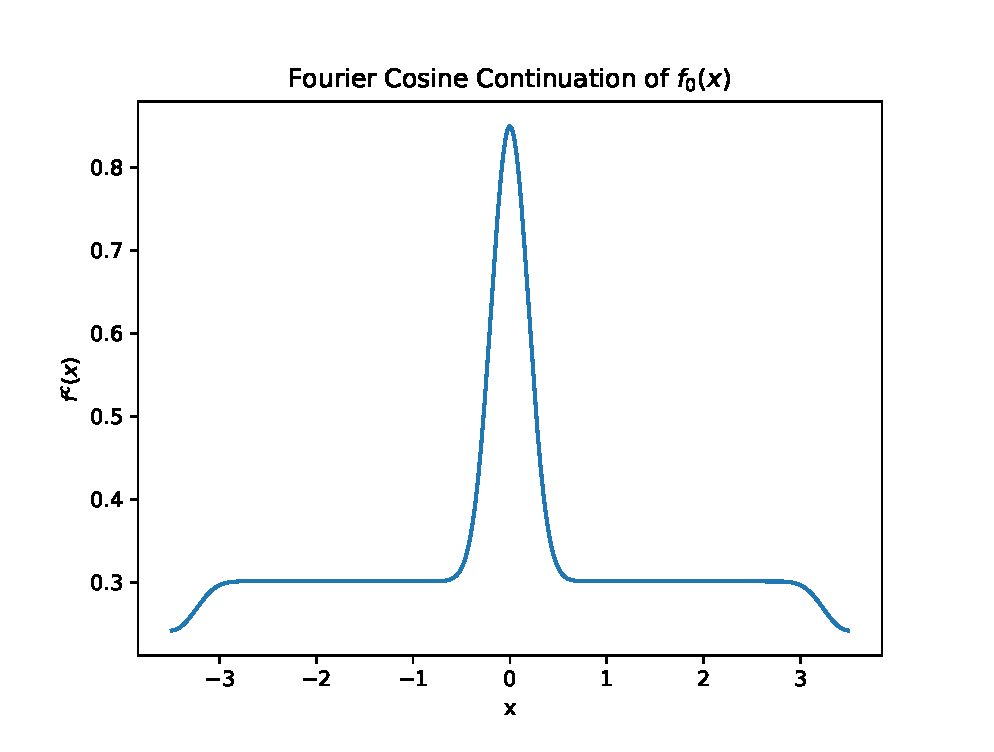
\includegraphics[scale=.5]{f_0Cosine.eps}
 \label{fig:Fig2}
&
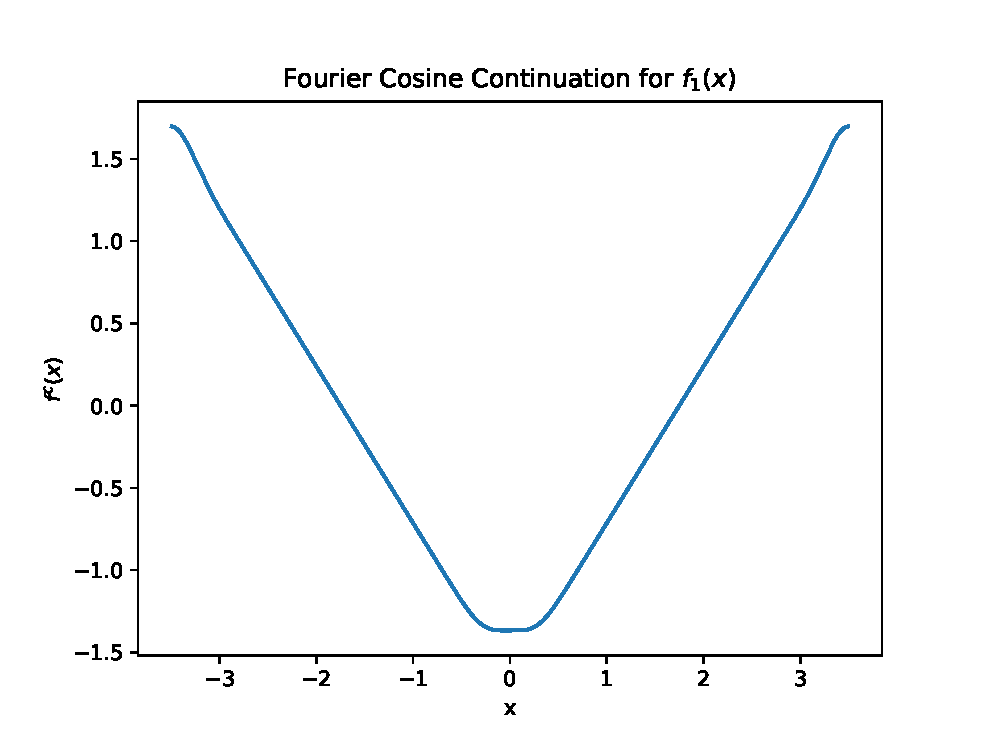
\includegraphics[scale=.5]{f_1Cosine.eps}
\label{fig:Fig3}
\\ \\
\hline


\end{tabular}
\caption{The first two polynomial approximations via Fourier Cosine Continuations}
\end{figure}




\begin{figure}

\begin{tabular}{|c|c|}
\hline
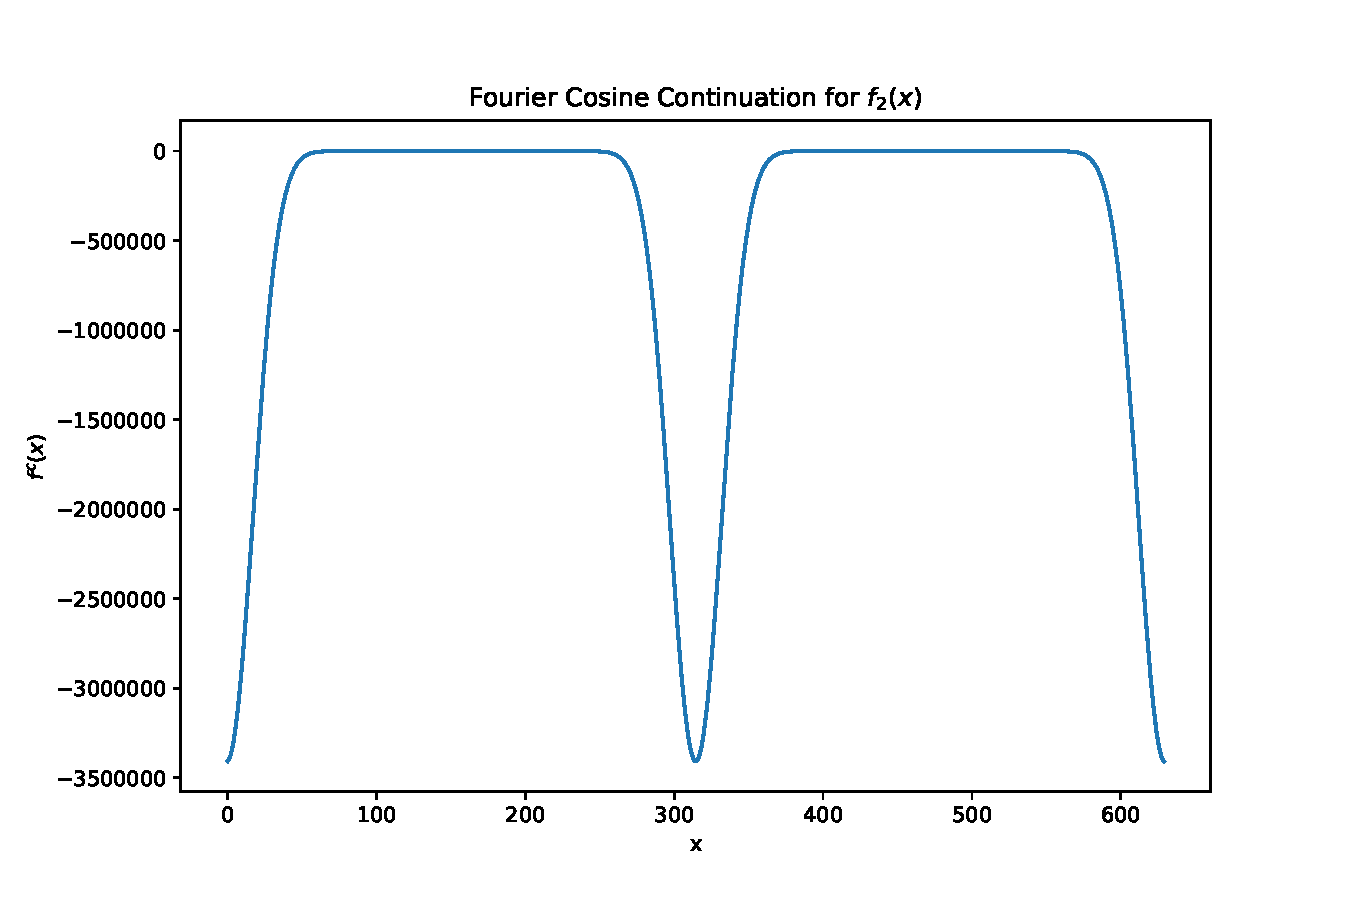
\includegraphics[scale=.3]{f_2Cosine.eps}
& 
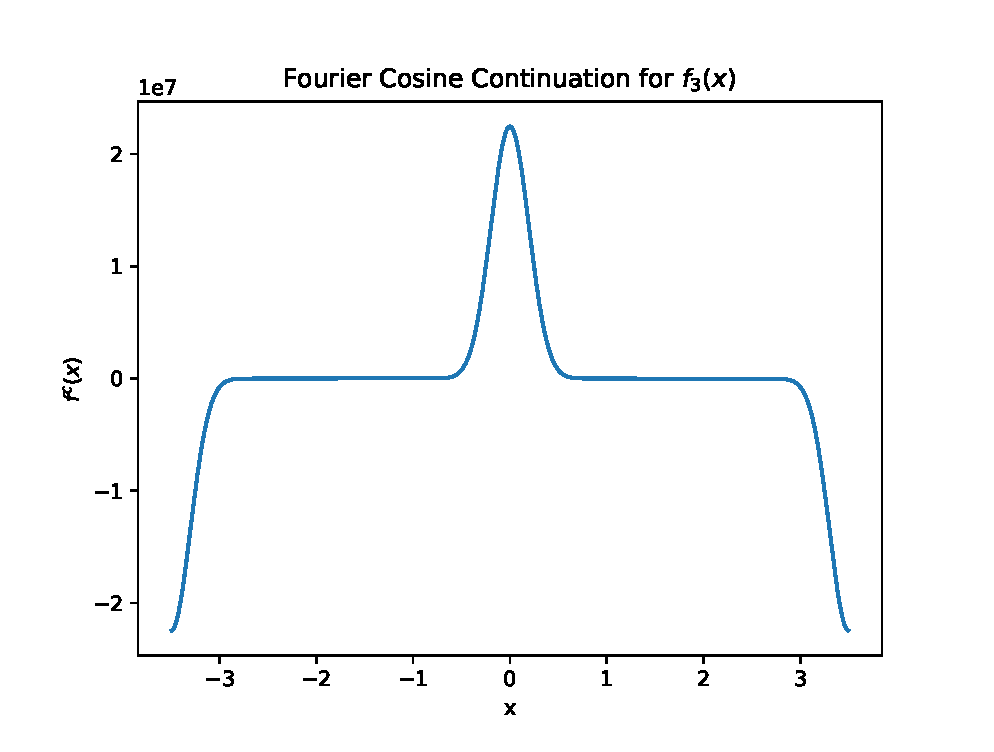
\includegraphics[scale=.4]{f_3Cosine.eps}
\\ \\
\hline
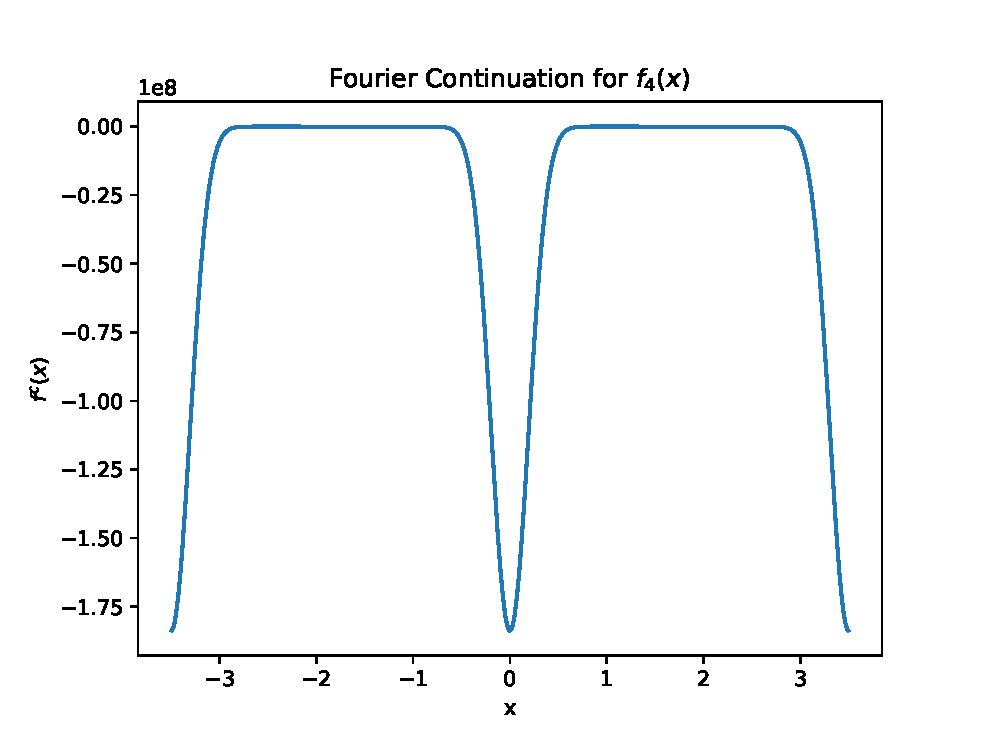
\includegraphics[scale=.4]{f_4Cosine.eps}
& 
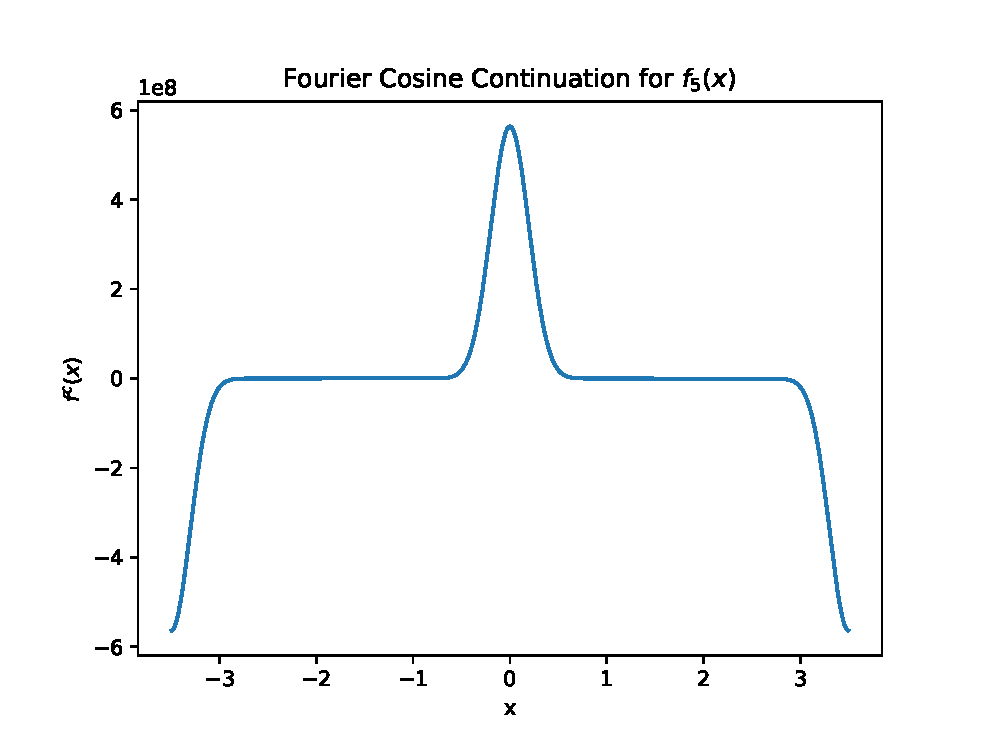
\includegraphics[scale=.4]{f_5Cosine.eps}
\\ \\
\hline
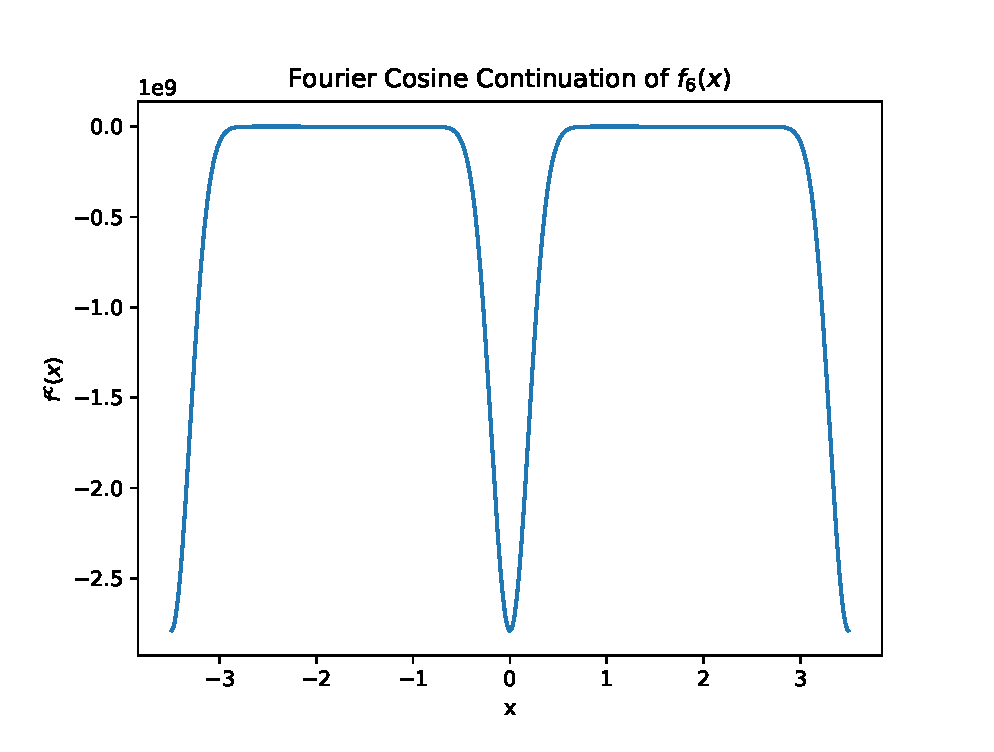
\includegraphics[scale=.4]{f_6Cosine.eps}
& 
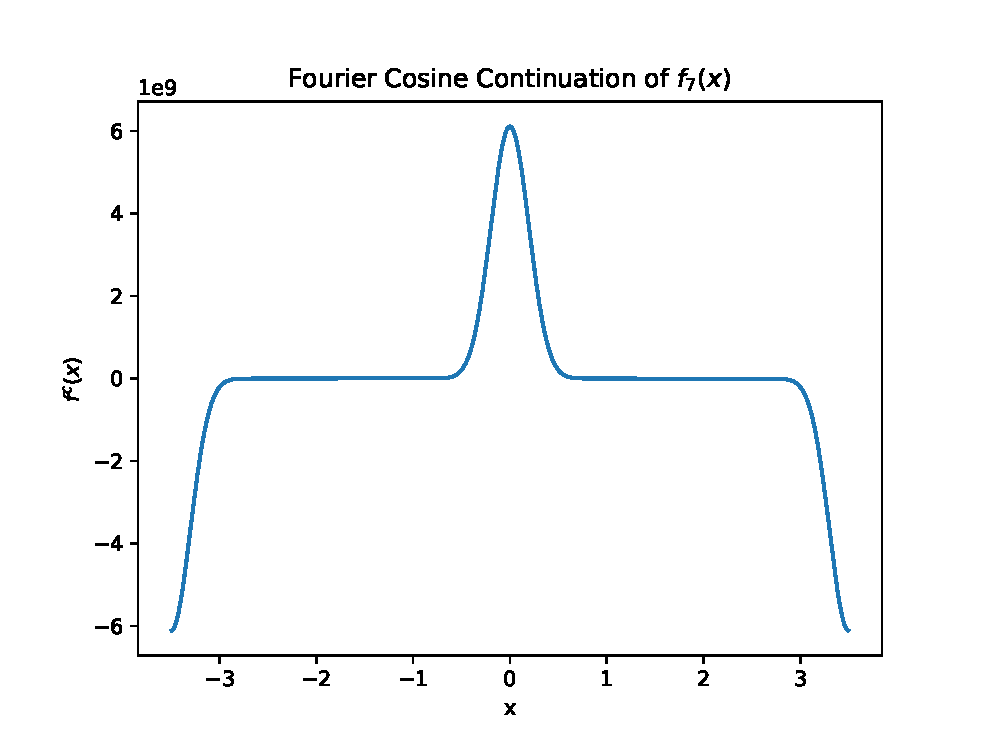
\includegraphics[scale=.4]{f_7Cosine.eps}
\\ \\
\hline
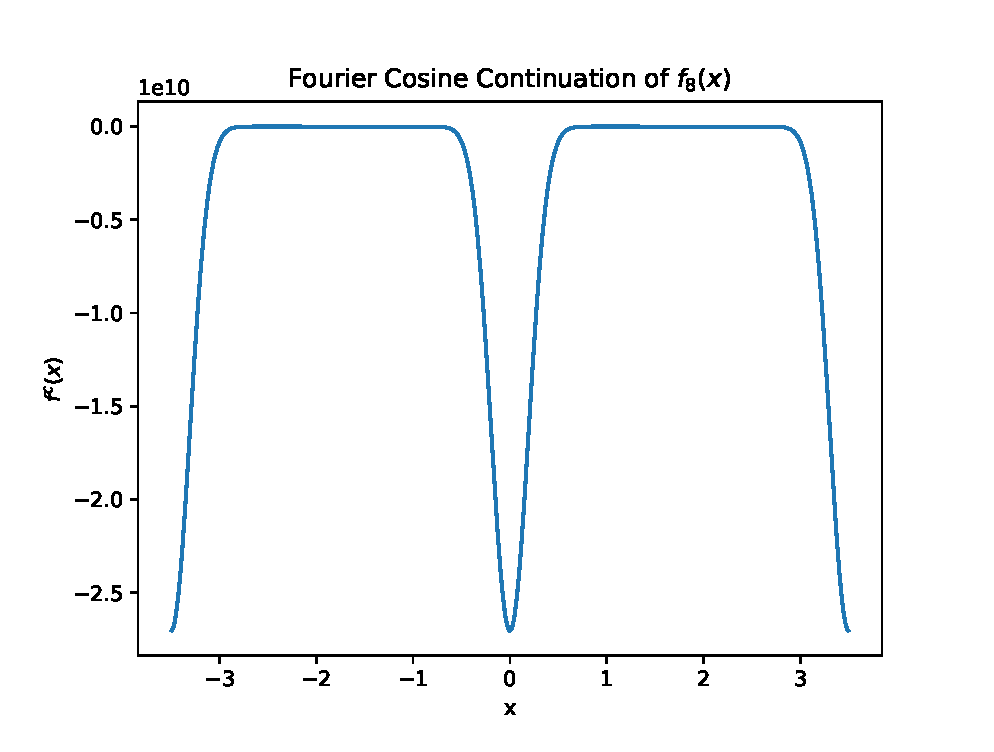
\includegraphics[scale=.4]{f_8Cosine.eps}
& 
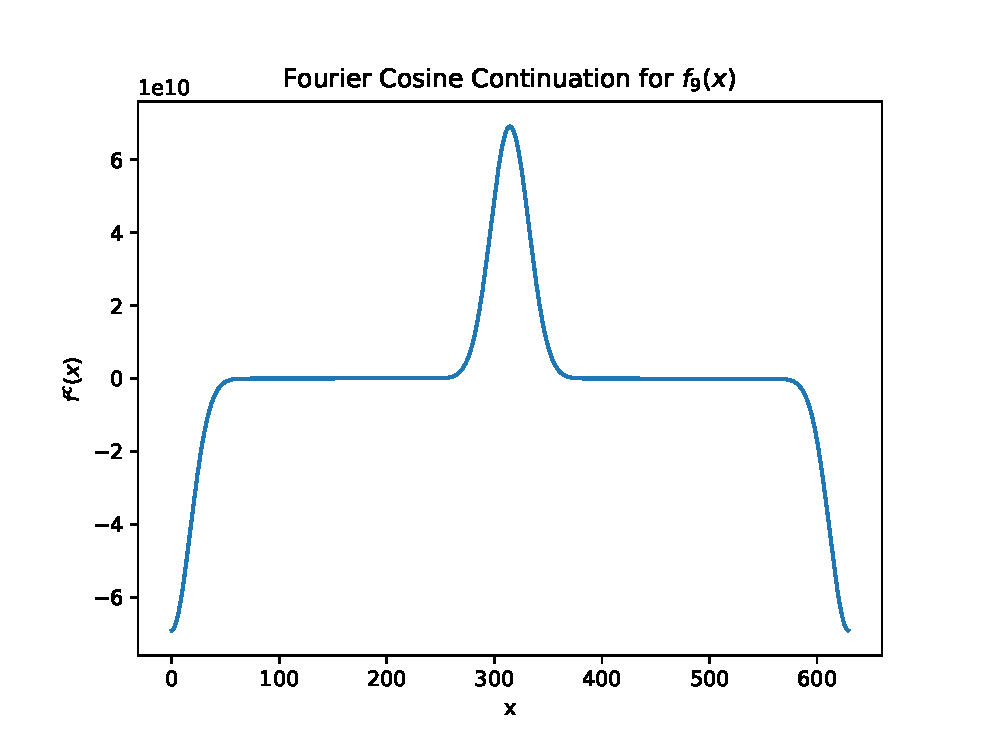
\includegraphics[scale=.4]{f_9Cosine.eps}
\\ \\



\end{tabular}
\caption{The last eight polynomial approximations via Fourier Cosine Continuations}
\end{figure}
\newpage 
The continuations themselves are large in magnitude but on the domain in question, match up to the original functions with great accuracy:
\begin{figure}[h!]
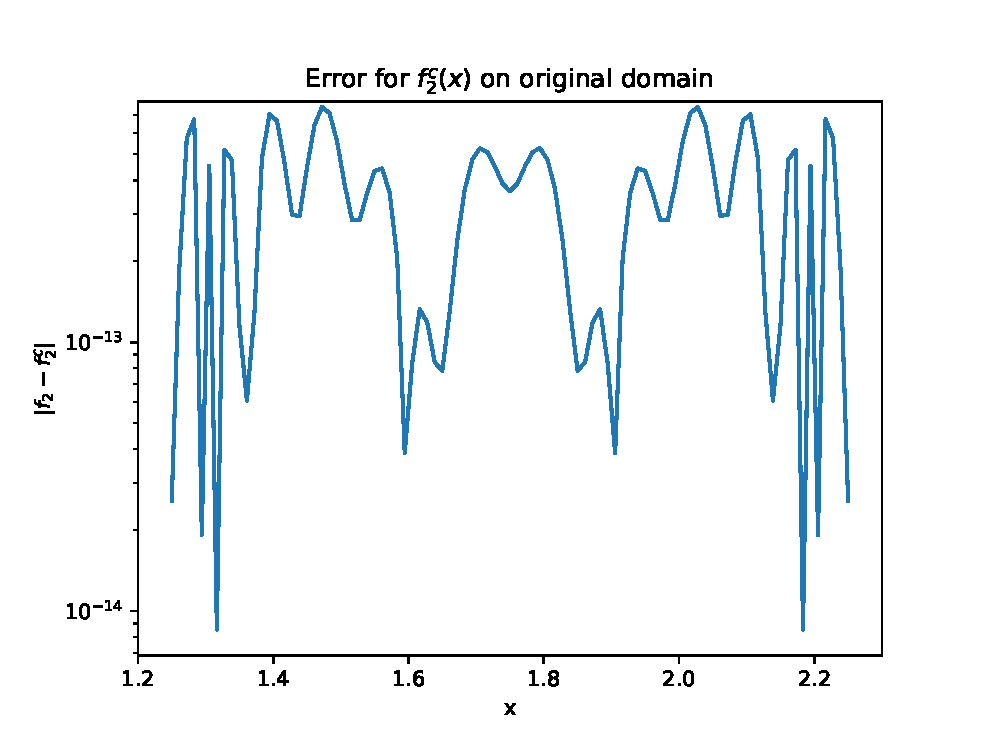
\includegraphics[scale=.5]{Error_f_2.eps}
\caption{The absolute error for the $2^{\text{nd}}$ degree polynomial on the original domain}
\end{figure}



Assuming $\mu = 0$, here are the computed $\lambda$ values and the respective accuracy and stability measures of the continuations for $\alpha = 0.001$. All values were computed in \texttt{BigFloat} to 77 digits but were truncated for legibility.   

\begin{tabular}{|c|c|c|c|}
\hline & & &\\
Degree & $\lambda$ & $\| f^c|_{\text{\tiny{fine grid}}}-f|_{\text{\tiny{fine grid}}}\|_2$ & $\dfrac{\|u|_{\text{\tiny{coarse grid}}}\|_2}{\|f|_{\text{\tiny{coarse grid}}}\|_2}$ \\ \hline  & & & \\
0 & $3.255881466810751\times 10^{-13}$ & $2.86510896623681\times 10^{-17}$ & $0.999999999999$ \\ \hline  & & &\\ 
1 & $1.839023251669854\times 10^{-13}$ & $3.92206770433105\times 10^{-17}$ & $0.999999999999$ \\ \hline  & & &\\
2 & $1.4852300108136326\times 10^{-10}$ &  $3.88957362362112\times 10^{-12}$ & $0.999999999999$ \\ \hline & & & \\
3 & $5.518469567738165\times 10^{-10}$ & $5.61719253880104\times 10^{-11}$ & $0.999999999999$ \\ \hline & & & \\
4 & $1.1767778737499883\times 10^{-9}$ & $2.0963541751156\times 10^{-10}$ & $0.999999999999$ \\ \hline & & & \\
5 & $3.0091447070493457\times 10^{-9}$ & $1.4098065193636\times 10^{-9}$ & $0.999999999999$ \\ \hline & & & \\
6 & $4.864688165149565\times 10^{-9}$ & $3.1835304451683\times 10^{-9}$ & $0.999999999999$ \\ \hline & & & \\
7 & $1.0373945031909215\times 10^{-8}$ & $1.52729276442667\times 10^{-8}$ &  $0.999999999999$ \\ \hline & & & \\
8 & $1.5639865553913073\times 10^{-8}$ & $3.08554433657289\times 10^{-8}$ & $0.999999999999$  \\ \hline & & & \\
9 & $3.071964692890429\times 10^{-8}$ & $1.72857119028618\times 10^{-7}$& $0.999999998446$  \\ \hline

\end{tabular}   
\\
\\


The goal here was to maintain the highest level of accuracy while still be stable up to a tolerance.  The continuations themselves were extremely large in magnitude, which cause issues when the continuations are implemented in the FC-Gram method in another programming language that only allows for 16 digits of precision.

We aim to find a better $\lambda$ which minimizes the maximum-norm of the continuation while maintaining stability, at the potential sacrifice of a few digits of accuracy, noting that this may involve adding another constraint to our system.


\section{Future Work} 
\subsection{Computational Work} 
The next step computationally is to take these continuations and try to find a functional relationship between the shape of the continuation and $\alpha$ for a given polynomial and build a basis of continuations for use in the FC-Gram method.  There also needs to be some form of predictor for the best values of $\lambda$ and $\mu$ in order to get a stable, high-accuracy approximation without having to bisect the values each time.

The sensitivity of the accuracy and stability for each polynomial approximation will be explored, based on both the value of $\alpha$ and the tolerance used to define something as stable in the bisection method.  Graphically, there should be some visual representation of the effect of $\lambda$ and $\mu$ and their combinations on accuracy and stability, especially for the higher-degree polynomials.  

Once the basis is stored, the FC-Gram method can be applied to test functions (like the Runge function) to test the accuracy limitations of the method for various numbers of points using FFTs.  This will give a good basis for comparison with other approximation methods.  Next, FFTs will be used to verify the accuracy of numerical derivatives on the continued functions, and then solve ODEs with initial data given by a test function.  A variety of boundary conditions beyond the zero boundary conditions enforced with the Green's Function will be tested.  

Lastly (for this particular approach) the FC-AD method will be implemented with the chosen ``best" continuations.  

There has been some trouble computationally with evaluating the Green's Function solution for small ($<0.001$) values of $\alpha$.  In order for this to be a fully implementable algorithm, any value of $\alpha$ must work, so an alternate computation for the Green's Function solutions will be used.  

Time permitting, we may try to use this attempt to solve other types of BVPs to see if we can induce stability by following the Green's function solutions to those problems.  

\subsection{Analytical Work} 
There will be analysis to justify results more formally.  
Specifically, the argument for a convergence estimate should be fully detailed.  In \cite{Platte}, it was proven that convergence is impossible for fast, stable approximations on equispaced points.  It will be shown that while the method doesn't actually achieve convergence from the continuation approximations to the function itself, high-accuracy results persist enough that convergence isn't an issue. In order to do this, the number of points used in the FC-Gram method will be increased and a maximal error estimate will be determined.   

A singular value analysis will demonstrate stability for the ``best" continuations found as the FC-Gram method is followed.   

We will use previous analytic results in \cite{FCAD2} combined with our numeric results to show that the FC-AD algorithm, when used in conjunction with our algorithm for Fourier Continuations, is stable. 
\newpage

\bibliographystyle{unsrt}
\bibliography{citations}



\end{document}  